\documentclass{article}

\usepackage{amsmath, amsfonts, microtype, xcolor, tikz, graphicx, hyperref, amsthm}
\usepackage[ruled, linesnumbered]{algorithm2e}
\usepackage[]{neurips_2019}

\newtheorem{theorem}{Theorem}

\SetKwComment{Comment}{$\triangleright$\ }{}

\usetikzlibrary{calc}

\tikzset{
    ncbar angle/.initial=90,
    ncbar/.style={
        to path=(\tikztostart)
        -- ($(\tikztostart)!#1!\pgfkeysvalueof{/tikz/ncbar angle}:(\tikztotarget)$)
        -- ($(\tikztotarget)!($(\tikztostart)!#1!\pgfkeysvalueof{/tikz/ncbar angle}:(\tikztotarget)$)!\pgfkeysvalueof{/tikz/ncbar angle}:(\tikztostart)$)
        -- (\tikztotarget)
    },
    ncbar/.default=0.5cm,
}

\tikzset{round left paren/.style={ncbar=0.5cm,out=110,in=-110}}
\tikzset{round right paren/.style={ncbar=0.5cm,out=70,in=-70}}

\title{Measuring causal influence with\\ back-to-back regression: the linear case}

\author{%
  Jean-Remi King\\
  CNRS\\
  \texttt{email} \\
  \And
  Fran\c{c}ois Charton\\
  Facebook AI\\
  \texttt{fcharton@fb.com}\\
  \And
  David Lopez-Paz\\
  Facebook AI\\
  \texttt{dlp@fb.com}
  \And
  Maxime Oquab\\
  Facebook AI\\
  \texttt{qas@fb.com}
}

\begin{document}

\maketitle

\begin{abstract}
Identifying causes from observations is at the core of science. This endeavor
is particularly challenging when i) potential factors are difficult to
manipulate individually and ii) observations are complex and multi-dimensional.
To address this issue, we introduce ``Back-to-Back'' regression (B2B), a
method designed to measure, from a set of co-varying factors, the causal
influences that most plausibly account for multidimensional observations. After
proving the consistency of B2B, we show that our method outperforms
least-squares and related regression and cross-decomposition techniques (e.g.
canonical correlation analysis and partial least squares) on two tasks: causal
identification and out-of-distribution prediction. Finally, we apply B2B to
neuroimaging recordings of 102 subjects reading word sequences. The results
show that the early and late brain responses caused by low- and high-level
word features respectively are more easily detected with B2B than with standard forward regression.
% conclude  open
\end{abstract}

\section{Introduction}

Natural sciences are tasked to find, from a set of hypothetical factors, the
minimal subset that suffices to reliably predict novel observations. This
endeavor is impeded by two major challenges.

First, causal and non-causal factors may be numerous and partially correlated.
% In physics,
% for example, one may be challenged to identify whether fusion is caused by a
% change in temperature or a change in pressure, as these two factors may, at
% first, be difficult to manipulate independently. This issue becomes increasingly
% pronounced as the number of potential factors increases.
In neuroscience, for
example, it can be challenging to identify whether word frequency modulates
brain activity during reading. Indeed, the
frequency of words in natural language covaries with other factors such as their
length (short words are more frequent than long words) and their categories
(determinants are more frequent than adverbs)
\citep{kutas2011thirty,pegado2014timing}. Instead of selecting a set of words
that controls for all of these factors simultaneously, it is thus common to use
a \emph{forward} "encoding model", i.e. to fit a linear regression to predict observations
(e.g. brain activity) from a minimal combination of competing factors (e.g.
word length, word frequency), and analytically investigate
the estimated contribution of each factor from the model's coefficients
\citep{friston1994statistical,naselaris2011encoding,weichwald2015causal,
king2018encoding,huth2016natural}.

The second challenge to measuring causal influence is that observations can be
multidimensional.
For example, brain activity is often
recorded with hundreds or thousands of simultaneous measurements via functional
Magnetic Resonance Imaging, magneto-encephalography (MEG) or multiple electro-
physiological probes \citep{friston1994statistical,steinmetz2018challenges}.
The relationship between putative causes and observations is thus often
done by training models in a \emph{backward}
fashion: i.e. from observations to putative causal factors. For example, it is
common to fit a support vector machine across multiple
brain voxels or multiple electrodes to detect the
category of a stimulus independently of common noise sources (e.g. head
movements, eye blink)
\citep{norman2006beyond,cichy2014resolving,
kriegeskorte2008representational, king2018encoding}.

Both \emph{forward} and \emph{backward} modeling have competing benefits and drawbacks.
Specifically, forward modeling disentangles the independent contribution of
correlated factors, but does not combine multidimensional observations. By
contrast, backward modeling combines multiple observations, but does not
disentangle factors that are linearly correlated \citep{weichwald2015causal,
hebart2018deconstructing, king2018encoding}. To combine some of the benefits of forward
and backward modeling, several authors have proposed to use cross-decomposition
techniques such as Partial Least Squares (PLS) and Canonical Correlation
Analysis (CCA) \citep{de2019multiway, bilenko2016pyrcca}. CCA and PLS aim to find, from two sets of
data $X$ and $Y$, the components $H$ and $G$ such that $XH$ and $YG$ are maximally
correlated or maximally covarying respectively.

While CCA and PLS can make use
of multidimensional features and observations, they are not designed
for feature discovery. First, these methods are not not directional: observations
and factors can be assigned to either $X$ or $Y$. Second, these method project $X$
and $Y$ onto a reduced but nonetheless multidimensional space. Third, because
CCA and PLS are based on a generalized eigen decomposition, their resulting
coefficients mix the features of $X$ and $Y$ in a way that makes them notoriously difficult to
interpret \citep{lebart1995statistique}.

Here, we introduce the `back-to-back regression' (B2B), which not only combines
the benefits of forward and backward modeling (Section~\ref{sec:algorithm}), but
can also provide robust, interpretable, unidimensional and unbiased coefficients for
each factor.

After detailing B2B and proving its convergence
(Section~\ref{sec:theorem}), we show with synthetic data that it outperforms
state-of-the-art forward, backward and cross-decomposition techniques in
disentangling causal factors (Section~\ref{sec:experiment_synthetic}). Finally,
we apply B2B to large neuroimaging datasets and reveal that distinct but
linearly-correlated word features lead to distinguishable brain representations
(Section~\ref{sec:experiment_real}).


\section{Back to back regression}
\label{sec:algorithm}


\begin{figure}[t!]
    \centering
    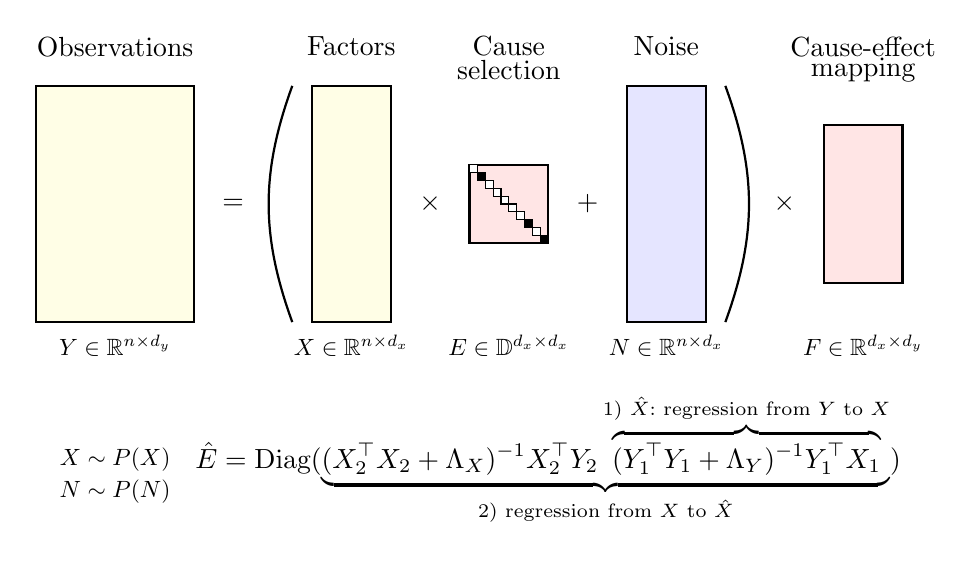
\begin{tikzpicture}
    \newcommand\posY{0}
    \newcommand\posX{3}
    \newcommand\posE{5}
    \newcommand\posN{7}
    \newcommand\posF{9.5}

    \node[thick, draw=black, minimum height=3cm, minimum width=2cm, fill=yellow!10] (Y) at (\posY, 0){};
    \node[] (eq) at (1.5, 0){$=$};
    \node[] (times) at (4, 0){$\times$};
    \node[thick, draw=black, minimum height=3cm, minimum width=1cm, fill=yellow!10] (X) at (\posX, 0){};
    \node[thick, draw=black, minimum height=1cm, minimum width=1cm, fill=red!10] (E) at (\posE, 0){};

    \draw[fill=white] (\posE - 0.5 + 0.0, 0.5 - 0.0) rectangle (\posE - 0.5 + 0.0 + 0.1, 0.5 - 0.0 - 0.1);
    \draw[fill=black] (\posE - 0.5 + 0.1, 0.5 - 0.1) rectangle (\posE - 0.5 + 0.1 + 0.1, 0.5 - 0.1 - 0.1);
    \draw[fill=white] (\posE - 0.5 + 0.2, 0.5 - 0.2) rectangle (\posE - 0.5 + 0.2 + 0.1, 0.5 - 0.2 - 0.1);
    \draw[fill=white] (\posE - 0.5 + 0.3, 0.5 - 0.3) rectangle (\posE - 0.5 + 0.3 + 0.1, 0.5 - 0.3 - 0.1);
    \draw[fill=white] (\posE - 0.5 + 0.4, 0.5 - 0.4) rectangle (\posE - 0.5 + 0.4 + 0.1, 0.5 - 0.4 - 0.1);
    \draw[fill=white] (\posE - 0.5 + 0.5, 0.5 - 0.5) rectangle (\posE - 0.5 + 0.5 + 0.1, 0.5 - 0.5 - 0.1);
    \draw[fill=white] (\posE - 0.5 + 0.6, 0.5 - 0.6) rectangle (\posE - 0.5 + 0.6 + 0.1, 0.5 - 0.6 - 0.1);
    \draw[fill=black] (\posE - 0.5 + 0.7, 0.5 - 0.7) rectangle (\posE - 0.5 + 0.7 + 0.1, 0.5 - 0.7 - 0.1);
    \draw[fill=white] (\posE - 0.5 + 0.8, 0.5 - 0.8) rectangle (\posE - 0.5 + 0.8 + 0.1, 0.5 - 0.8 - 0.1);
    \draw[fill=black] (\posE - 0.5 + 0.9, 0.5 - 0.9) rectangle (\posE - 0.5 + 0.9 + 0.1, 0.5 - 0.9 - 0.1);

    \node[] (plus) at (6, 0){$+$};
    \node[thick, draw=black, minimum height=3cm, minimum width=1cm, fill=blue!10] (N) at (\posN, 0){};
    \node[thick, draw=black, minimum height=2cm, minimum width=1cm, fill=red!10] (F) at (\posF, 0){};
    \draw [thick] (2.25, -1.5) to [round left paren ] (2.25, 1.5);
    \draw [thick] (7.75, -1.5) to [round right paren ] (7.75, 1.5);

    \node[] (times2) at (8.5, 0){$\times$};

    \node[] (annY) at (\posY, -1.8){\scalebox{0.85}{$Y \in \mathbb{R}^{n \times d_y}$}};
    \node[] (annX) at (\posX, -1.8){\scalebox{0.85}{$X \in \mathbb{R}^{n \times d_x}$}};
    \node[] (annE) at (\posE, -1.8){\scalebox{0.85}{$E \in \mathbb{D}^{d_x \times d_x}$}};
    \node[] (annN) at (\posN, -1.8){\scalebox{0.85}{$N \in \mathbb{R}^{n \times d_x}$}};
    \node[] (annF) at (\posF, -1.8){\scalebox{0.85}{$F \in \mathbb{R}^{d_x \times d_y}$}};

    \node[] (labY) at (\posY, 2){Observations};
    \node[] (labX) at (\posX, 2){Factors};
    \node[] (labE) at (\posE, 2){Cause};
    \node[] (labE) at (\posE, 1.7){selection};
    \node[] (labN) at (\posN, 2){Noise};
    \node[] (labF) at (\posF, 2){Cause-effect};
    \node[] (labF) at (\posF, 1.7){mapping};

    \node[] (sim1) at (0,-3.25) {\scalebox{0.85}{$X \sim P(X)$}};
    \node[] (sim2) at (0,-3.65) {\scalebox{0.85}{$N \sim P(N)$}};
    \node[] (reg1) at (5.5,-3.25) {$\hat{E} = \text{Diag}(\underbrace{(X_2^\top X_2 + \Lambda_X)^{-1} X_2^\top Y_2\overbrace{(Y_1^\top Y_1 + \Lambda_Y)^{-1} Y_1^\top X_1}^{\text{1) } \hat{X} : \text{ regression from } Y \text{ to } X}}_{\text{2) regression from } X \text{ to } \hat{X}})$};
    \end{tikzpicture}
    \caption{Back-to-back regression identifies the subset of factors $E_{ii} = 1$ in $X$ that influence some observations $Y$ by 1) regressing from $Y$ to $X$ to obtain $\hat{X}$, and ii) returning the diagonal of the regression coefficients from $X$ to $\hat{X}$.}
    \label{fig:b2b}
\end{figure}

We consider the measurement of multivariate signal $Y$, generated from a set of variables $X$, via some unknown linear apparatus $F$.
%
Not all the variables in $X$ exert a causal influence on $Y$.
%
By considering a square binary diagonal matrix of \emph{causal influences} $E$, we denote by $XE$ the causal factors of $Y$.
%
In summary, our model can be formalized as:
%
\begin{equation}
    Y = (XE + N)F,\label{eq:model}
\end{equation}
%
where $N$ is a centered, unobserved noise variable.
%
While the triplet of variables $X$ and $N$ are independent, we allow each of them to have a general covariance matrix.
%
In practice, we observe $n$ samples $(X, Y)$ from the model.
%
This process, along with the sizes of all variables involved, is illustrated in Figure~\ref{fig:b2b}.
%
Given the model in Equation~\eqref{eq:model}, \textbf{the goal} of Back-to-Back Regression (B2B) is to estimate the matrix of causal influences $E$.

\subsection{Algorithm}


Back-to-Back Regression (B2B) consists of two steps.
%
First, we estimate the linear regression coefficients $\hat G$ from $Y$ to $X$, and construct the predictions $\hat X = Y \hat G$.
%
This backward regression recovers the correlations between $Y$ and each factor of $X$.
%
Second, we estimate the linear regression coefficients $\hat H$ from $X$ to $\hat X$.
%
The diagonal of the regression coefficients $\hat H$, denoted by $\hat{E} = \text{Diag}(\hat{H})$, is the desired estimate of the causal influence matrix $E$.

If using regularized least-squares, arguably the most commonly employed linear regression technique \citep{hoerl1959optimum, rifkin2007notes}, the solution of B2B has a closed form solution:
\begin{align}
    \hat G &= (Y^\top Y + \Lambda_Y)^{-1} Y^\top X,\label{eq:solG}\\
    \hat H &=(X^\top X + \Lambda_X)^{-1} X^\top Y \hat G,\label{eq:solH}
\end{align}
%
where $\Lambda_X$ and $\Lambda_Y$ are two diagonal matrices of regularization parameters, useful to invert the covariance matrices of $X$ and $Y$ if these are ill-conditioned.

Performing two regressions over the same data sample can result in overfitting, as spurious correlations in the data absorbed by the first regression will be leveraged by the second one.
%
To avoid this issue, we split our sample $(X, Y)$ at random into two equally-sized halves $(X_1, Y_1)$ and $(X_2, Y_2)$.
%
Then, the first regression is performed using $(X_1, Y_1)$, and the second regression is performed using $(X_2, Y_2)$.
%
To compensate for the reduction in sample size caused by the split, B2B is repeated over many random splits, and the final estimate $\hat E$ of the causal influence matrix is the average over the estimates associated to each split \citep{efron1992bootstrap}.
%
After obtaining $\hat{E}$, we can fit a final regression from $X \hat{E}$ to $Y$.

We summarize the B2B procedure in Algorithm~\ref{algorithm:b2br}.
%
The rest of this section provides a theoretical guarantee on the correctness of B2B, and an optional post-processing step to binarize the estimated causal influence matrix.



\begin{algorithm}[H]
    %\SetAlgoLined
    \KwIn{input data $X \in \mathbb{R}^{n \times d_x}$, output data $Y \in \mathbb{R}^{n\times d_y}$, number of repetitions $m \in \mathbb{N}$.}
    \KwOut{estimate of causal influences $\hat{E} \in \mathbb{D}^{d_x \times d_x}$.}
    $\hat{E} \leftarrow 0$\;
    \For{$i = 1, \ldots, m$}{
        $(X, Y) \leftarrow \text{ShuffleRows}((X, Y))$\;
        $(X_1, Y_1), (X_2, Y_2) \leftarrow \text{SplitRowsInHalf}((X, Y))$\;
        $\hat{G} = \text{LinearRegression}(Y_1, X_1)$ \Comment*[r]{$\hat G = (Y_1^\top Y_1 + \Lambda_Y)^{-1} Y_1^\top X_1$}
        $\hat{H} = \text{LinearRegression}(X_2, Y_2 \hat{G})$ \Comment*[r]{$\hat H=(X_2^\top X_2 + \Lambda_X)^{-1} X_2^\top Y_2 \hat G$}
        $\hat{E} \leftarrow \hat{E} + \text{Diag}(\hat{H})$\;
    }
    $\hat{E} \leftarrow \hat{E} / m$\;
    $\hat{W} \leftarrow \text{LinearRegression}(X \hat{E}, Y)$\;
    \Return{$\hat{E}$, $\hat{W}$}
    \caption{Back-to-back regression.}
    \label{algorithm:b2br}
\end{algorithm}

\subsection{Theoretical guarantees}
\label{sec:theorem}

\begin{theorem}[B2B consistency - general case]

     Consider the B2B model from Equation $Y = (XE + N)F$, $N$ centred and full rank noise.
     %
     If $F$ and $X$ are full-rank on $Img(E)$, then, the solution of B2B, $\hat H$, will minimise
     %
     $\min_H  \left \| X - XH\right\| ^2  + \left \| NH\right \| ^2$and satisfy $E\hat H = \hat H$
\end{theorem}
\begin{proof}

 Let $\hat G$ and $\hat H$ be the solutions of the first and second regressions of B2B, we have
 \begin{align*}
    \hat G = \arg \min_G \mathbb{E}[\left \| YG - X \right \|^2] &=   \arg \min_G \mathbb{E}[\left \| X - (XE + N)FG \right\|^2]\\
%                                                        &{}= \arg \min_G \mathbb{E}[\left \| X - XEFG\right\| ^2]  + \mathbb{E}[\left \| NFG\right \| ^2]\\
                                                        &{}= \arg \min_G \left \| X - XEFG\right\| ^2  + \left \| NFG\right \| ^2
     \label{eq:doublenorm}
\end{align*}
\begin{align*}
    \hat H = \arg \min_H \mathbb{E}[\| XH - Y \hat{G} \|^2] &=\arg  \min_H \mathbb{E}[\| XH - (XE + N)F \hat G \|^2] \\
    &=\arg \min_H \mathbb{E}[\| X(H - EF \hat G) \| ^2] + \mathbb{E}[\| NF\hat G \| ^2]\\
%    &= \arg \min_H \mathbb{E}[\| X(H - EF \hat G) \| ^2]\\
    &= EF \hat G
\end{align*}

Let us prove that $EF\hat G = F\hat G$, that is, that the $d_x$ bottom rows of $F\hat G$ are zero. Let $Z=F^\dagger EF\hat G$. We have $FZ = FF^\dagger EF  \hat G= EF\hat G$ ($FF^\dagger E =E$ since $F$ is full rank on $Img(E)$). Since E is a contraction, we have $ \| NEF\hat G\|^2 \leq \| NF\hat G \|^2$. Therefore, 
 $$\left \| X - XEFZ\right \| ^2  + \left \| NFZ\right \| ^2 = \| X - XEF\hat G \| ^2  + \| NEF\hat G \| ^2 \leq \| X - XEF\hat G \| ^2  + \| NF\hat G \| ^2$$

But as $\hat G =  \arg \min_G \left \| X - XEFG\right\| ^2  + \left \| NFG\right \| ^2$, the above inequality is an equality, $Z=\hat G$ and $EF\hat G = F\Hat G$. Therefore, $\left \| X - XEFG\right \| ^2  + \left \| NFG\right \| ^2 = \left \| X - XEFG\right \| ^2  + \left \| NEFG\right \| ^2 = \left \| X - XH\right \| ^2  + \left \| NH\right \| ^2$ is minimised by $\hat G$ and $\hat H$. Finally, $E\hat H = E EF\hat G = EF\hat G = \hat H$. This completes the proof.
\end{proof}

So, $\hat H = \arg \min_H  \left \| X - XEH\right\| ^2  + \left \| NEH\right \| ^2 = (E X^\top XE +EN^\top NE) ^\dagger EXX^\top$.

Assuming, without loss of generality, that the active features are the $k$ first, we have 

$X^\top X = \left(\begin{array}{lccl}\Sigma_{X1} & \Sigma_{X2} \\ \Sigma_{X2} & \Sigma_{X3}\end{array}\right)$, $N^\top N = \left(\begin{array}{lccl}\Sigma_{N1} & \Sigma_{N2} \\ \Sigma_{N2} & \Sigma_{N3}\end{array}\right)$ and

$\hat H = \left(\begin{array}{cc}(\Sigma_{X1}+\Sigma_{N1})^{-1}\Sigma_{X1} & (\Sigma_{X1}+\Sigma_{N1})^{-1}\Sigma_{X2} \\0 & 0\end{array}\right)$

$Diag_k (\hat H) = Diag((\Sigma_{X1}+\Sigma_{N1})^{-1}\Sigma_{X1}) = Diag((I+\Sigma_{X1}^{-1}\Sigma_{N1})^{-1})$

In the absence of noise, we have $Diag(\hat H) = Diag(E)$. Else the k first diagonal elements of $\hat H$ are all positive, and bounded by $\frac{\sigma_{X_k}}{\sigma_{X_k} +\sigma_{N_1}}$ and $\frac{\sigma_{X_1}}{\sigma_{X_1} +\sigma_{N_k}}$, where  $\sigma_{X_1}$, $\sigma_{X_k}$, $\sigma_{N_1}$ and $\sigma_{N_k}$ denote the largest and smallest eigenvalues of $\Sigma_{X1}$ and $\Sigma_{N1}$. 

The average value of the coefficients of $Diag(\hat H)$ is the trace of $\hat H$ divided by k. On average, since $X$ and $N$ are not correlated, $\Sigma_{X1}^{-1}\Sigma_{N1}$ should have a low condition numbers, and $\frac{Var(X)}{Var(X)+Var(N)}$ provide a good estimate of $\frac{1}{k}Tr(\hat H)$.

\subsection{Binarizing $\hat{E}$}

On the one hand, we have leveraged B2B to obtain the estimate $\hat{E}$, which is a diagonal matrix with real entries.
%
On the other hand, the true causal influence matrix $E$ is a binary matrix, which hard-selects the causal factors of $Y$ from $X$.
%
In this section, we provide one of the many possible recipes to binarize $\hat{E}$ and estimate the collection of causal factors.

In regression analysis, the traditional approach to this problem employs a $t$-test to check whether the regression coefficients differ from zero \citep{student1908probable}.
%
However, this test will not succeed here, since the estimate $\hat{E}$ is obtained from a double regression, and any employed regularization will add a bias to the diagonal of $\hat{E}$.
%
Instead, we treat the binarization of $\hat{E}$ as a clustering problem: separate the elements in the diagonal into a group of ``small values'', and a group of ``large values''.
%
More specifically, we propose to maximize the ratio of inter-group variance and to minimize the intra-group variance, over all possible splits of the diagonal into $p$ largest values and $d_x-p$ smallest values.
%
Letting $m_0$ and $m_1$ be the average values of the two clusters, $p$ and $d_x-p$ their size, and $v$ the total variance of the sample, we select the split maximizing the Sonquist-Morgan \citep{sonquist_morgan} criterion $\frac{p(d_x-p)}{d_x} \frac{(m_1 - m_0)^2}{v}$.
%
To binarize $\hat{E}$, set to one all the $p$ diagonal entries belonging to the ``large values'' group in the decided split, and setting to zero the rest of the $d_x-p$ diagonal entries.

\section{Experiments}

We perform two experiments to evaluate the performance of B2B: one on controlled synthetic data, and a second one on a real, large-scale magneto-encephalography dataset.
%
We use scikit-learn \citep{sklearn}.

\subsection{Synthetic data}
\label{sec:experiment_synthetic}

We evaluate the performance of B2B throughout a series of experiments on
controlled synthetic data.
%
The purpose of these experiments is to evaluate the ability of B2B on its
ability to 1) recover causal factors when the ground truth is known and 2)
accurately predict independent and identically distributed data otherwise.

The data generating process for each experiment constructs $m=1000$ training examples
according to the model $Y = (\text{h} XS + N)F$, where $\text{h}$ is a
scalar that modulates the signal-to-noise ratio.
%
Here,
%\begin{itemize} \item $F \in \mathbb{R}^{d_x \times d_y}$ contains entries
%drawn from $\mathcal{N}(0, \sigma^2)$, \item $X \in \mathbb{R}^{m \times d_x}$
%contains rows drawn from $\mathcal{N}(0, \Sigma_X)$, \item $N \in \mathbb{R}^{m
%\times d_x}$ contains rows drawn from $\mathcal{N}(0, \Sigma_N)$, \item $S \in
%\mathbb{R}^{d_x \times d_x}$ is a binary diagonal matrix containing $n_c$ ones,
%\item $\Sigma_X = AA^\top$, where $A \in \mathbb{R}^{d_x \times d_x}$ contains
%entries drawn from $\mathcal{N}(0, \sigma^2)$, \item $\Sigma_N = BB^\top$,
%where $B \in \mathbb{R}^{d_x \times d_x}$ contains entries drawn from
%$\mathcal{N}(0, \sigma^2)$, \end{itemize}
    $F \in \mathbb{R}^{d_x \times d_y}$ contains entries drawn from
$\mathcal{N}(0, \sigma^2)$ where $\sigma^2$ is inversely proportional to $d_x$,
$X \in \mathbb{R}^{m \times d_x}$ contains rows
drawn from $\mathcal{N}(0, \Sigma_X)$, $N \in \mathbb{R}^{m \times d_x}$
contains rows drawn from $\mathcal{N}(0, \Sigma_N)$, $S \in \mathbb{R}^{d_x
\times d_x}$ is a binary diagonal matrix containing $n_c$ ones, $\Sigma_X =
AA^\top$ where $A \in \mathbb{R}^{d_x \times d_x}$ contains entries drawn from
$\mathcal{N}(0, \sigma^2)$, $\Sigma_N = BB^\top$ where $B \in \mathbb{R}^{d_x
\times d_x}$ contains entries drawn from $\mathcal{N}(0, \sigma^2)$, and the
factor $\text{h} \in \mathcal{R}_+$.

To simulate a wide range of experimental conditions, we sample 10 values in log-space for $d_x, d_y \in \left[ 10, 100 \right]$, $n_c \in \left[ 3, 63 \right]$,
$\text{h} \in \left[ 0.001, 10 \right]$. We discard the cases where $n_c > d_x$, limit $d_x, d_y$ to 100 to keep the running time under 2 hours for each condition, and average over 5 random seeds.
%
% Each condition is simulated under $5$ different random seeds.

We compare the performance of B2B against four baseline methods.
%
% To be updated

\subsubsection{Baseline models}

All baseline methods were based on the implementations of scikit-learn \citep{sklearn} and Pyrcca
\citep{bilenko2016Pyrcca}. For pedagogical purposes, we briefly summarize them below.

Forward regression consists of an $l2$-regularized "ridge" regression from the
putative causes $X$ to the observations $Y$: \begin{equation} H_{fwd} = (X^T X
+\lambda I)^{-1} X^T Y \end{equation}

Backward regression consists of an $l2$-regularized "ridge" regression from $Y$
to $X$: \begin{equation} G_{bwd} = (Y^T Y +\lambda I)^{-1} Y^T X \end{equation}

CCA finds $G_{cca}\in\mathbb{R}^{d_z, d_y}$ and $H_{cca}\in\mathbb{R}^{d_z, d_x}$
% such that
s.t.
$X$ and $Y$ are maximally correlated in a latent $Z$ space:
% \begin{equation} maxcorr(XH^T, YG^T) \end{equation}
\begin{equation} G_{cca},H_{cca} = \argmax_{G,H} corr(XH^T, YG^T) \end{equation}

% To be checked
PLS finds $G_{pls}\in\mathbb{R}^{d_z, d_y}$ and $H_{pls}\in\mathbb{R}^{d_z, d_x}$
% such that
s.t.
$X$ and $Y$ are maximally covarying in a latent $Z$ space:
% \begin{equation} maxcov(XH^T, YG^T) \end{equation}
\begin{equation} G_{pls},H_{pls} = \argmax_{G,H} \text{cov}(XH^T, YG^T) \end{equation}

We employ five-fold nested cross-validation to select the optimal number of components
for CCA and PLS. Regressions were $\ell2$-regularized with a $\lambda$ regularization
parameters fitted with the efficient leave-one-out procedure implemented in
scikit-learn RidgeCV \citep{sklearn}.

\subsubsection{Evaluating Causal Discovery from models' coefficients}

%
B2B leads to \emph{scalar} coefficients for non-causal
features. The diagonal of this matrix, $\hat S \in \mathbb{R}^{d_x}$, can thus be directly used
as a causal contribution estimate. Note that this estimate is unbiased (i.e.
zeros-centered) only if the second regression $H$ is not regularized.

In contrast, the loading coefficients of the Forward ($H_i \in \mathbb{R}^{d_y}$),
Backward ($G^i \in \mathbb{R}^{d_y}$), CCA and PLS models ($H_i \in \mathbb{R}^{d_z}$) lead to a
loading \emph{vector} for each feature $i$.
To estimate causal contribution, we must thus transform such vectors into
scalars, by e.g. taking the sum of square coefficients:
% \begin{equation}
  $\hat S_i = \sum_j {H^j_i}^2 $
% \end{equation}
Note that in such B2B cases, the estimates are thus positive and would thus bias
a second-level statistical analysis against 0.

Finally, to estimate whether each model accurately identifies causal factors independently of
their potential biases, we compute the
area-under-the-curve (AUC) across factors $AUC(S, \hat S)$.
%\begin{equation} AUC = 1 - \sum_1^m (S_k - S_{k-1}) ( \hat{S}_k +
%\hat{S}_{k-1}) / 2 \end{equation}
By definition, this AUC evaluation can only be done when ground truth labels are available, as is the case in
this synthetic setup, but not in the neuroimaging experiments below.

Figures~\ref{fig:percondition} (top) and~\ref{fig:auc_plots} (top) show the
results of this AUC evaluation. Note that the figure does not display each
feature separately, as they are randomly generated. The results show that B2B
compares favorably to other methods on these synthetic data.


\begin{figure}[t]
  \centering
  \includegraphics[width=\linewidth]{figures/auc_condition.pdf}
  \includegraphics[width=\linewidth]{figures/r_in_condition.pdf}
  \vspace{-4ex}
  \caption{Synthetic experiments. Average AUC (top) and Feature Importance
  $\Delta R$ (bottom) when varying experimental conditions individually.
  Higher is better. B2B compares favorably in all cases.
  \label{fig:percondition}}
\end{figure}


\subsubsection{Evaluating Causal Discovery through the reliability of held-out prediction}

In most real-world cases, $S$ is not known. Consequently, the above AUC
evaluation cannot be estimated.
To address this issue, we assess the ability of each model to reliably predict
independent and identically distributed data from $Y$, given all of the $X$
features versus all-but-one feature $X_{-i}$ (i.e. 'knock-out X'). This
procedure results in two correlation metrics $R_{full}$ and $R_{knockout}$ for
each feature (for the B2B and Backward models) for each dimension of $Y$ (for
the Forward model) or each canonical dimension of $Y$ (for CCA and PLS). The
difference $\Delta R_i = R_{full}-R_{knockout}$ indicates how much each
$X_i$ improves the prediction of
a) the target dimension (i.e. $G^iY \in \mathbb{R}$ for B2B,
b) the average across all of the dimensions $j$ of $Y$
($\frac{1}{d_y}\sum_{j}^{d_y}\Delta R_i^{j}$) for the
Forward model or
c) the average across the canonical dimensions $j$ of $Y$
($\frac{1}{d_z}\sum_{j}^{d_z}\Delta R_i^{j}$) for CCA and PLS.
We show in Appendix~\ref{appendix:feature_importance} pseudo-code to assess
feature importance for each model. For the Backward Model, feature importance
cannot be assessed as the $X$ collinearity is never
taken into account.

Figures~\ref{fig:percondition} (bottom) and~\ref{fig:auc_plots} (right, in
Appendix) show the results of this evaluation on held-out data.
Overall both the AUC and the held-out prediction reliability evaluations
show that B2B compares favorably to the baseline models.


\subsection{Magnetoencephalography data}
\label{sec:experiment_real}

\subsection{The MOUS dataset}

Next, we apply our method to brain imaging data, on the ``Mother Of Unification
Studies'' (MOUS) dataset \cite{schoffelen2019204}. The dataset consists of
anonymized multimodal neuroimaging data that has been acquired from 204 healthy
human subjects, which participated in either a auditory or a visual version of a
language experiment. In this work, we use the subset corresponding to the visual
variant recorded using magneto-encephalography (MEG).

Subjects were presented a set of 120 sentences in Dutch, and a scrambled lists
of the same words for a controlled experiment. Each word was presented on a
screen for no less than 300 ms and no more than 1400ms, 351 ms on average.
Successive words were separated by an empty screen for 300ms, and successive
sentences were separated by an empty screen for a few (3-4) seconds.

The data contains the timestamp for each word presentation, allowing to align
time series to stimuli onsets for all words.

As a result, we obtain, for each of the 301 sensors and each word presented, a
time series of 67 real-values spanning $\left[-100ms, 1500ms\right]$ relative to
the stimulus onset. Each of the 102 subjects (we used data from 93 subjects) was
presented approximately 2700 words during the experiment.


\subsection{Application of the method}





\section{Related work}

In the context of neuroimaging, the first regression of B2B relates to the first step of Representational Similarity Analysis (RSA) \citep{kriegeskorte2008representational}. Indeed, RSA analyzes the similarity of brain responses associated with specific conditions (e.g. distinct images), by (1) fitting one-against-all classifiers on each condition and (2) testing whether these classifiers can discriminate all other conditions. The resulting confusion matrix can then be analyzed in an unsupervised manner to reveal that some conditions lead to similar brain activity patterns. B2B differs from RSA in that (1) it uses regressions instead of classifications, and can thus generalize to new contexts and (2)
it is fully supervised.

More generally, B2B is related to CCA \citep{cca_hotelling}, but departs from it in four main aspects. First, CCA performs an additional eigenvector decomposition of what would be the $H$ coefficients in B2B \eqref{eq:solH}. Second, CCA does not typically optimize two distinct regularization parameters. Third, CCA does not use bagging between $G$ and $H$. Finally, CCA does not diagonalize nor binarize the $H$ matrix to estimate $\hat E$. More generally, CCA aims to find maximally correlated components between $X$ and $Y$, and does not assume any causal direction. By contrast, B2B assumes that $X$ causes $Y$. Together, these differences may explain why B2B can reliably outperform CCA on estimating causal influences and predicting $Y$ in novel environments (Fig. \ref{table:synthetic}).

B2B is also related to, but different from usual causal discovery algorithms \citep{peters2017elements} that hypothesize on the direction of causality, or from measures of causal influence requiring time information \citep{granger1969investigating, janzing2013quantifying}.
%
B2B seems to have a similar flavour to half-sibling regression \citep{scholkopf2016modeling}, in the sense that we observe a large number of variables corrupted by the same source of noise; we leave the study of the precise link between these two models for future work.


\section{Conclusion}
In this work, we proposed Back-to-Back Regression (B2BR), a method to 
measure the causal influence of a potential set of variables generating some observations.
%
B2BR performs two successive multidimensional regressions: one from the output domain, and another one from the input domain.
%
We provided a theoretical guarantee about the consistency of B2BR, and compared it to several baselines in controlled synthetic experiments.
%
We also applied B2BR to a recent brain imaging dataset, analyzing the timing
of brain responses and their connection to word features.
%
We obtained results consistent with prior work in neuroscience literature, confirming the efficacy of B2BR for real data analysis.


\clearpage
\newpage

\bibliographystyle{plain}
\bibliography{paper}

% \documentclass{article}

\usepackage{amsmath, amsfonts, microtype, xcolor, tikz, graphicx, hyperref, amsthm}
\usepackage[ruled, linesnumbered]{algorithm2e}
\usepackage[]{neurips_2019}
\newtheorem{theorem}{Theorem}


\title{Measuring causal influence with\\ back-to-back regression: the linear case - supplementary material}

\begin{document}

\appendix

\maketitle


\section{Theorem - detailed proof}
\label{sec:theorem}

\begin{theorem}[B2B consistency - general case]

     Consider the B2B model from Equation $$Y = (XE + N)F$$ $N$ centred and full rank noise.

     If $F$ and $X$ are full-rank on $Img(E)$, then, the solution of B2B, $\hat H$, will minimise

     $$\min_H  \left \| X - XH\right\| ^2  + \left \| NH\right \| ^2$$ and satisfy

     $$E\hat H = \hat H$$
\end{theorem}
\begin{proof}

 Let $\hat G$ and $\hat H$ be the solutions of the first and second regressions of B2B.

 Since $\hat G$ is the least square estimator of $X$ from $Y$
 \begin{align*}
    \hat G = \arg \min_G \mathbb{E}[\left \| YG - X \right \|^2]
\end{align*}
Replacing $Y$ by its model definition $Y = (XE+N)F$, we have
 \begin{align*}
    \hat G &=   \arg \min_G \mathbb{E}[\left \| X - (XE + N)FG \right\|^2] =\arg \min_G \mathbb{E}[\left \| X - XEFG + NFG \right\|^2]
  \end{align*}
  Since $N$ is centered and independent of $X$, we have
  \begin{align}
    	  \hat G &=  \arg \min_G \left \| X - XEFG\right\| ^2  + \left \| NFG\right \| ^2
     \label{eq:Gdoublenorm}
\end{align}

Samely, for $\hat H$, we have
\begin{align*}
    \hat H = \arg \min_H \mathbb{E}[\| XH - Y \hat{G} \|^2] &=\arg  \min_H \mathbb{E}[\| XH - (XE + N)F \hat G \|^2] \\
    &=\arg \min_H \mathbb{E}[\| X(H - EF \hat G) \| ^2] + \mathbb{E}[\| NF\hat G \| ^2]\\
    &= \arg \min_H \mathbb{E}[\| X(H - EF \hat G) \| ^2]
 \end{align*}
 a positive quantity which reaches a minimum (zero) for
 \begin{align}
    \hat H = EF \hat G
    \label{eq:Hdoublenom}
\end{align}

Let us now prove that $EF\hat G = F\hat G$.

Let $F^\dagger$ be the pseudo inverse of $F$, and $Z=F^\dagger EF\hat G$, we have $FZ = FF^\dagger EF \hat G$

Since $F$ is full rank on $Img(E)$, we have $FF^\dagger E =E$, and $FZ = EF\hat G$

As $E$ is a binary diagonal matrix, it is an orthogonal projection and therefore a contraction, thus
 $$ \| NEF\hat G\|^2 \leq \| NF\hat G \|^2$$ and
 $$\left \| X - XEFZ\right \| ^2  + \left \| NFZ\right \| ^2 = \| X - XEF\hat G \| ^2  + \| NEF\hat G \| ^2 \leq \| X - XEF\hat G \| ^2  + \| NF\hat G \| ^2$$

But since $\hat G =  \arg \min_G \left \| X - XEFG\right\| ^2  + \left \| NFG\right \| ^2$, we also have
$$\left \| X - XEF\hat G\right\| ^2  + \left \| NF\hat G\right \| ^2 \leq \left \| X - XEFZ\right \| ^2  + \left \| NFZ\right \| ^2$$

Summarizing the above,
$$\left \| X - XEF\hat G\right\| ^2  + \left \| NF\hat G\right \| ^2 \leq \| X - XEF\hat G \| ^2  + \| NEF\hat G \| ^2 \leq \| X - XEF\hat G \| ^2  + \| NF\hat G \| ^2$$
$$\left \| X - XEF\hat G\right\| ^2  + \left \| NF\hat G\right \| ^2 = \| X - XEF\hat G \| ^2  + \| NEF\hat G \| ^2$$
$$\left \| NF\hat G\right \| ^2 =  \| NEF\hat G \| ^2$$

$N$ being full rank, this yields $EF\hat G = F\Hat G$.

Replacing into $\eqref{eq:Gdoublenorm}$, and setting $H = EFG$, we have
\begin{align*}
	\hat G &=  \arg \min_G  \left \| X - XEFG\right \| ^2  + \left \| NFG\right \| ^2 \\
	&=   \arg \min_G \left \| X - XEFG\right \| ^2  + \left \| NEFG\right \| ^2 \\
	\hat H &=  \arg \min_H \left \| X - XH\right \| ^2  + \left \| NH\right \| ^2
	\label{eq:4}
\end{align*}

Finally, $E\hat H = E EF\hat G = EF\hat G = \hat H$, since $E$, a binary diagonal matrix, is involutive. This completes the proof.
\end{proof}



\end{document}


%\section{Appendices}
%
%This should hold part of the tests, explanations on simulation, detailed results and stuff on meg data

\end{document}
